\documentclass[11pt,a4paper]{article}

% ─── fonts ────────────────────────────────────────────────────────────────
\usepackage{fontspec}
\setmainfont{Inter}
\newfontfamily\titlefont{Sometype Mono}
\newfontfamily\monofont{Sometype Mono}

% ─── geometry & layout ────────────────────────────────────────────────────
\usepackage[a4paper, margin=2.4cm, top=2.6cm, bottom=2.6cm]{geometry}
\usepackage{xcolor}
% — text & background —
\definecolor{ink}{HTML}{111111}
\definecolor{paper}{HTML}{FFFFFF}
\definecolor{muted}{HTML}{666666}
\definecolor{rule}{HTML}{DADADA}
% — semantic accent palette (coral / teal / amber / forest) —
\definecolor{coral}{HTML}{C9442B}      % primary highlight, recommendations
\definecolor{coraltint}{HTML}{FBEAE3}  % soft fill for coral callouts
\definecolor{teal}{HTML}{1F7A85}       % concepts, methods, pipelines
\definecolor{tealtint}{HTML}{E3F1F3}
\definecolor{amber}{HTML}{B97A1B}      % risks, warnings, open questions
\definecolor{ambertint}{HTML}{F8EFDD}
\definecolor{forest}{HTML}{3E7A52}     % verified, recommended, "do this"
\definecolor{foresttint}{HTML}{E4EFE6}
% legacy aliases used elsewhere in the file
\colorlet{accent}{coral}
\colorlet{box}{coraltint}
\pagecolor{paper}
\color{ink}

% ─── titles ───────────────────────────────────────────────────────────────
\usepackage{titlesec}
\titleformat{\section}
  {\titlefont\Large\bfseries\color{ink}}{\thesection}{0.6em}{}[\vspace{-0.4em}\textcolor{rule}{\hrule height 0.6pt}]
\titleformat{\subsection}
  {\titlefont\large\bfseries\color{ink}}{\thesubsection}{0.5em}{}
\titlespacing*{\section}{0pt}{1.6em}{0.6em}
\titlespacing*{\subsection}{0pt}{1.0em}{0.3em}

% ─── headers / footers ────────────────────────────────────────────────────
\usepackage{fancyhdr}
\pagestyle{fancy}
\fancyhf{}
\renewcommand{\headrulewidth}{0pt}
\fancyfoot[L]{{\titlefont\footnotesize ETH ROBOTICS CLUB}}
\fancyfoot[R]{{\titlefont\footnotesize \thepage}}
\fancyfoot[C]{{\titlefont\footnotesize\color{muted}DATASET STRATEGY \,|\, GATE DETECTION}}

% ─── tables ───────────────────────────────────────────────────────────────
\usepackage{booktabs}
\usepackage{tabularx}
\usepackage{array}
\newcolumntype{L}[1]{>{\raggedright\arraybackslash}p{#1}}

% ─── callouts ─────────────────────────────────────────────────────────────
\usepackage[most]{tcolorbox}
% Default style (coral) used by \begin{tcolorbox}[title=...].
\tcbset{
  colback=coraltint, colframe=coral, boxrule=0pt, leftrule=2.4pt,
  arc=0pt, outer arc=0pt,
  fonttitle=\titlefont\bfseries\color{coral},
  coltitle=coral,
  left=10pt, right=10pt, top=8pt, bottom=8pt,
  enhanced, breakable,
}
% Coloured semantic variants — invoke as
%   \begin{tcolorbox}[concept,  title=...]
%   \begin{tcolorbox}[risk,     title=...]
%   \begin{tcolorbox}[verified, title=...]
\tcbset{
  concept/.style ={colback=tealtint,   colframe=teal,
                   fonttitle=\titlefont\bfseries\color{teal},   coltitle=teal},
  risk/.style    ={colback=ambertint,  colframe=amber,
                   fonttitle=\titlefont\bfseries\color{amber},  coltitle=amber},
  verified/.style={colback=foresttint, colframe=forest,
                   fonttitle=\titlefont\bfseries\color{forest}, coltitle=forest},
}

% ─── lists ────────────────────────────────────────────────────────────────
\usepackage{enumitem}
\setlist{leftmargin=1.2em, topsep=0.3em, itemsep=0.2em, parsep=0pt}

% ─── graphics & links ─────────────────────────────────────────────────────
\usepackage{graphicx}
\usepackage{tikz}
\usetikzlibrary{calc, arrows.meta, positioning, shapes.geometric, shapes.misc, fit, backgrounds, decorations.pathreplacing}
\usepackage{pgfplots}
\pgfplotsset{compat=1.18}
\usepackage[hidelinks]{hyperref}
\hypersetup{
  colorlinks=true,
  linkcolor=ink,
  urlcolor=accent,
  citecolor=ink,
}

% ─── dotted-drone cover watermark ─────────────────────────────────────────
% Inspired by ESRA's dotted-Europe hero treatment: a uniform grid of small
% dots clipped to a top-down quadcopter silhouette (central body, four
% diagonal arms in an X, four propeller circles).
%
% Geometry (TikZ units, 1 unit = 1cm by default):
%   body        rounded square, half-side B around origin
%   propellers  four circles centred on (R, R), (-R, R), (-R, -R), (R, -R)
%   arms        thick rotated rectangles connecting body corners to props
\newcommand{\DroneDotWatermark}{%
  \begin{tikzpicture}[overlay, remember picture]
  % shift slightly down of page centre so the title block sits cleanly over
  % the body of the drone, with propellers framing top-bottom-left-right.
  \begin{scope}[shift={($(current page.center)+(0,-2.6cm)$)}, scale=1.40]
    \begin{scope}
      \clip
        % central body — slightly rounded square
        [rounded corners=6pt] (-1.8,-1.8) rectangle (1.8,1.8) [sharp corners]
        % propellers — circle on each diagonal at radius R=4.6
        ({4.6/sqrt(2)},  {4.6/sqrt(2)})  circle (2.05)
        ({-4.6/sqrt(2)}, {4.6/sqrt(2)})  circle (2.05)
        ({4.6/sqrt(2)},  {-4.6/sqrt(2)}) circle (2.05)
        ({-4.6/sqrt(2)}, {-4.6/sqrt(2)}) circle (2.05)
        % arms — fatter rectangles (half-width 0.85) connecting body to props
        % NE arm: body-NW corner -> outer-NW -> outer-SE -> body-SE
        (0.20, 1.65) -- ({4.6/sqrt(2) - 0.85}, {4.6/sqrt(2) + 0.85}) --
        ({4.6/sqrt(2) + 0.85}, {4.6/sqrt(2) - 0.85}) -- (1.65, 0.20) -- cycle
        % NW arm
        (-1.65, 0.20) -- ({-4.6/sqrt(2) - 0.85}, {4.6/sqrt(2) - 0.85}) --
        ({-4.6/sqrt(2) + 0.85}, {4.6/sqrt(2) + 0.85}) -- (-0.20, 1.65) -- cycle
        % SE arm
        (1.65, -0.20) -- ({4.6/sqrt(2) + 0.85}, {-4.6/sqrt(2) + 0.85}) --
        ({4.6/sqrt(2) - 0.85}, {-4.6/sqrt(2) - 0.85}) -- (0.20, -1.65) -- cycle
        % SW arm
        (-0.20, -1.65) -- ({-4.6/sqrt(2) + 0.85}, {-4.6/sqrt(2) - 0.85}) --
        ({-4.6/sqrt(2) - 0.85}, {-4.6/sqrt(2) + 0.85}) -- (-1.65, -0.20) -- cycle;
      % tighter dot grid for halftone density
      \foreach \x in {-8.4,-8.13,...,8.4}{
        \foreach \y in {-8.4,-8.13,...,8.4}{
          \fill[ink, opacity=0.20] (\x,\y) circle (0.052);
        }
      }
    \end{scope}
  \end{scope}
  \end{tikzpicture}%
}

% ─── bibliography ─────────────────────────────────────────────────────────
\usepackage[backend=biber,style=numeric-comp,sorting=none,maxbibnames=4]{biblatex}
\addbibresource{refs.bib}

% ─── misc ─────────────────────────────────────────────────────────────────
\usepackage{microtype}
\usepackage{xurl}                       % allow URL line-breaks at any character
\setlength{\parskip}{0.5em}
\setlength{\parindent}{0pt}
\setlength{\emergencystretch}{1.6em}     % prevent overfull from rigid line breaks
\hyphenpenalty=800

\providecommand{\degree}{\textdegree}
% \code{...} renders inline paths/identifiers in Sometype Mono and allows
% line-breaks at any character — this is what kills overfull hboxes when a
% long path lands at the end of a line.
\DeclareUrlCommand{\code}{\urlstyle{tt}\monofont\small\color{ink}}

% ─── figures ──────────────────────────────────────────────────────────────
% Fig 1: Domain gap — twin bar charts side-by-side comparing detection rate
% and reprojection error on the TII test split vs real recorded footage.
\newcommand{\FigDomainGap}{%
\begin{figure}[!ht]
\centering
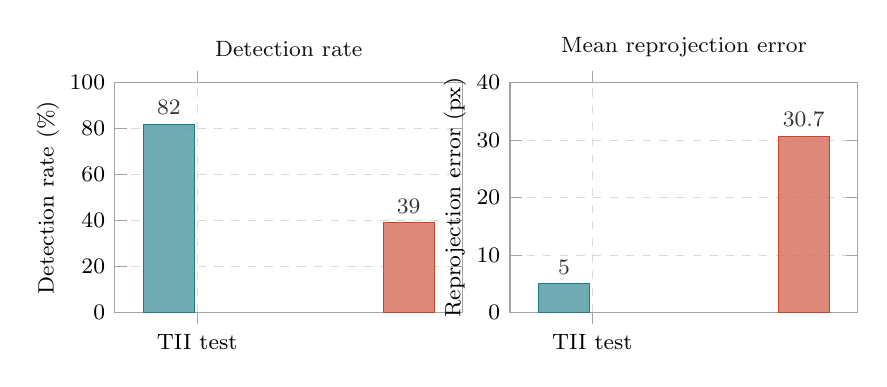
\begin{tikzpicture}
  \begin{axis}[
    name=plotL, width=6.0cm, height=4.5cm,
    ybar, bar width=0.65cm, enlarge x limits=0.45,
    ymin=0, ymax=100,
    ylabel={\footnotesize Detection rate (\%)},
    ylabel style={yshift=-0.3em},
    symbolic x coords={TII test, Real footage},
    xtick=data,
    nodes near coords,
    nodes near coords style={font=\footnotesize\titlefont, color=ink},
    every node near coord/.append style={anchor=south},
    tick label style={font=\footnotesize},
    axis line style={color=muted!60},
    tick style={color=muted!60},
    grid=major, major grid style={dashed, color=rule},
    title={\titlefont\footnotesize\color{ink} Detection rate},
  ]
    \addplot[fill=teal!75,   draw=teal,  fill opacity=0.85] coordinates {(TII test,82)};
    \addplot[fill=coral!75,  draw=coral, fill opacity=0.85] coordinates {(Real footage,39)};
  \end{axis}
  \begin{axis}[
    at={(plotL.south east)}, anchor=south west, xshift=0.6cm,
    width=6.0cm, height=4.5cm,
    ybar, bar width=0.65cm, enlarge x limits=0.45,
    ymin=0, ymax=40,
    ylabel={\footnotesize Reprojection error (px)},
    ylabel style={yshift=-0.3em},
    symbolic x coords={TII test, Real footage},
    xtick=data,
    nodes near coords,
    nodes near coords style={font=\footnotesize\titlefont, color=ink},
    every node near coord/.append style={anchor=south},
    tick label style={font=\footnotesize},
    axis line style={color=muted!60},
    tick style={color=muted!60},
    grid=major, major grid style={dashed, color=rule},
    title={\titlefont\footnotesize\color{ink} Mean reprojection error},
  ]
    \addplot[fill=teal!75,   draw=teal,  fill opacity=0.85] coordinates {(TII test,5.0)};
    \addplot[fill=coral!75,  draw=coral, fill opacity=0.85] coordinates {(Real footage,30.7)};
  \end{axis}
\end{tikzpicture}
\caption*{\footnotesize\textbf{Figure 1.} The domain gap that motivates this brief. Same checkpoint, two evaluation sets:
the TII test split (teal) and our team's real recorded footage (coral). Detection rate halves and reprojection error grows
$6\times$. Source numbers: \code{README.md} \S Known Issues, lines 31--48.}
\label{fig:domain-gap}
\end{figure}%
}

% Fig 2: Detection pipeline — RGB image -> segmentation -> mask ->
% QuAdGate corner extraction -> PnP -> 6-DoF pose. Mirrors MonoRace Fig 5
% \cite{bahnam2026monorace} and what our repo actually runs.
\tikzset{
  pipenode/.style ={draw, line width=0.7pt, rounded corners=2pt,
                    minimum width=2.0cm, minimum height=1.0cm,
                    align=center, font=\footnotesize, inner sep=4pt},
  pipein/.style   ={pipenode, draw=muted, fill=rule!30, text=ink},
  pipelearn/.style={pipenode, draw=coral, fill=coraltint, text=ink},
  pipeclass/.style={pipenode, draw=teal,  fill=tealtint,  text=ink},
  pipeout/.style  ={pipenode, draw=forest, fill=foresttint, text=ink},
  pipearrow/.style={-{Stealth[length=4pt, width=4pt]}, line width=0.7pt, color=muted!90},
}
\newcommand{\FigPipeline}{%
\begin{figure}[!ht]
\centering
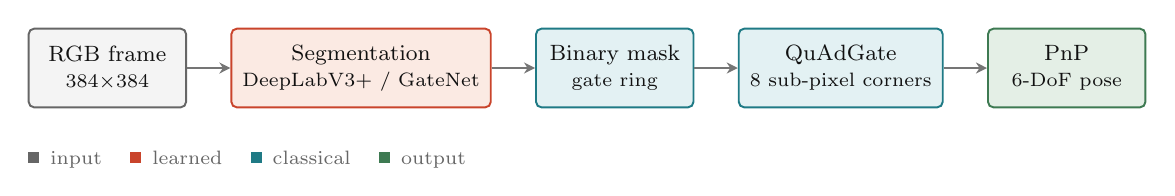
\begin{tikzpicture}[node distance=0.55cm]
  \node[pipein]    (img)  {RGB frame\\ \scriptsize $384{\times}384$};
  \node[pipelearn, right=of img]  (seg)  {Segmentation\\ \scriptsize DeepLabV3$+$ / GateNet};
  \node[pipeclass, right=of seg]  (mask) {Binary mask\\ \scriptsize gate ring};
  \node[pipeclass, right=of mask] (corn) {QuAdGate\\ \scriptsize 8 sub-pixel corners};
  \node[pipeout,   right=of corn] (pnp)  {PnP\\ \scriptsize 6-DoF pose};
  \draw[pipearrow] (img)  -- (seg);
  \draw[pipearrow] (seg)  -- (mask);
  \draw[pipearrow] (mask) -- (corn);
  \draw[pipearrow] (corn) -- (pnp);
  % legend strip
  \node[anchor=west, font=\scriptsize\color{muted}, inner sep=0pt] at ($(img.south west)+(0,-0.65cm)$)
    {\textcolor{muted}{\rule[0.18ex]{0.5em}{0.5em}}\, input \hspace{0.6em}
     \textcolor{coral}{\rule[0.18ex]{0.5em}{0.5em}}\, learned \hspace{0.6em}
     \textcolor{teal}{\rule[0.18ex]{0.5em}{0.5em}}\, classical \hspace{0.6em}
     \textcolor{forest}{\rule[0.18ex]{0.5em}{0.5em}}\, output};
\end{tikzpicture}
\caption*{\footnotesize\textbf{Figure 2.} The two-stage gate-detection pipeline used in this repo. The learned segmentation
backbone runs once per frame; QuAdGate then extracts sub-pixel inner and outer corners by intersecting LSD line segments and
matching descriptors. The structure mirrors the A2RL-winning MonoRace pipeline (Fig.~5 of~\cite{bahnam2026monorace}).}
\label{fig:pipeline}
\end{figure}%
}

% Fig 3: Three-tier evaluation pyramid — TII held-out (top, fastest),
% real-footage benchmark (middle), on-site smoke test (bottom, definitive).
\newcommand{\FigEvalTiers}{%
\begin{figure}[!ht]
\centering
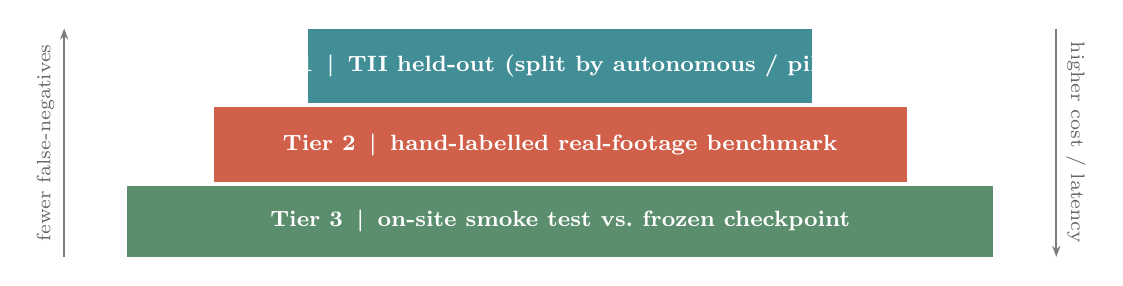
\begin{tikzpicture}[font=\footnotesize]
  \def\rh{0.95}      % row height
  \def\gap{0.05}     % gap between rows
  % Tier 1 — narrowest band on top (cheap, fast feedback)
  \fill[teal!85]   (-3.2,2*\rh+\gap)   rectangle ( 3.2,3*\rh+\gap);
  \node[white, font=\footnotesize\bfseries] at (0,2.5*\rh+\gap) {Tier 1 \,\textbar\, TII held-out (split by autonomous / piloted)};
  % Tier 2 — middle (slower, venue-relevant)
  \fill[coral!85]  (-4.4,1*\rh)        rectangle ( 4.4,2*\rh);
  \node[white, font=\footnotesize\bfseries] at (0,1.5*\rh) {Tier 2 \,\textbar\, hand-labelled real-footage benchmark};
  % Tier 3 — widest at bottom (slowest, definitive)
  \fill[forest!85] (-5.5,0)            rectangle ( 5.5,1*\rh-\gap);
  \node[white, font=\footnotesize\bfseries] at (0,0.5*\rh-\gap/2) {Tier 3 \,\textbar\, on-site smoke test vs.\ frozen checkpoint};
  % side annotations: speed (left), cost (right)
  \draw[-{Stealth[length=4pt]}, color=muted!85, line width=0.6pt]
       (-6.3,0) -- (-6.3,3*\rh+\gap) node[midway, sloped, above, color=muted, font=\scriptsize] {fewer false-negatives};
  \draw[-{Stealth[length=4pt]}, color=muted!85, line width=0.6pt]
       (6.3,3*\rh+\gap) -- (6.3,0) node[midway, sloped, above, color=muted, font=\scriptsize] {higher cost / latency};
\end{tikzpicture}
\caption*{\footnotesize\textbf{Figure 3.} Three-tier evaluation. Each tier catches failure modes the cheaper one cannot:
TII held-out catches segmentation regressions; the real-footage benchmark catches the domain shift the brief is built around;
the on-site smoke test catches venue-specific surprises. A checkpoint advances only after all three pass.}
\label{fig:eval-tiers}
\end{figure}%
}

% Fig 4: Fine-tuning protocol — frozen encoder, tunable decoder + last 2
% conv blocks, with a 1:1 rehearsal mini-batch from TII to prevent
% catastrophic forgetting (rationale: \cite{qiao2024continual}).
\newcommand{\FigFineTune}{%
\begin{figure}[!ht]
\centering
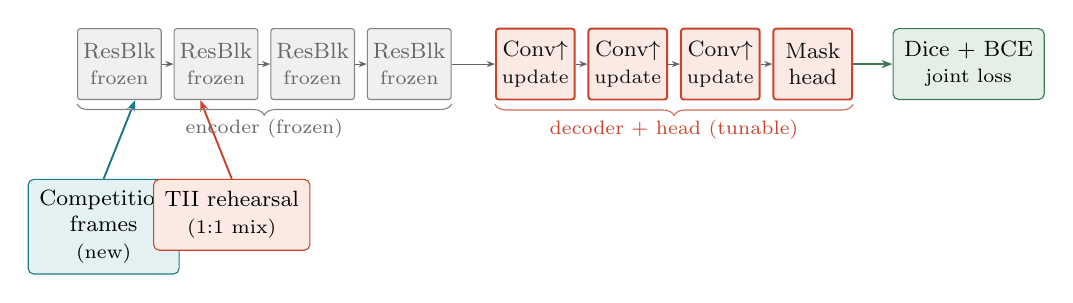
\begin{tikzpicture}[
  font=\footnotesize,
  layer/.style={draw, rounded corners=1pt, minimum width=1.0cm, minimum height=0.9cm, align=center, inner sep=2pt},
  frozen/.style={layer, draw=muted!80, fill=rule!40, text=muted},
  tunable/.style={layer, draw=coral, fill=coraltint, text=ink, line width=0.7pt},
  databox/.style={draw, rounded corners=2pt, align=center, font=\footnotesize, inner sep=4pt, minimum height=0.9cm},
]
  % network: encoder (4 frozen layers) + decoder (4 tunable layers) + head
  \node[frozen]                (e1)                {ResBlk\\ \scriptsize frozen};
  \node[frozen, right=0.15cm of e1]  (e2)          {ResBlk\\ \scriptsize frozen};
  \node[frozen, right=0.15cm of e2]  (e3)          {ResBlk\\ \scriptsize frozen};
  \node[frozen, right=0.15cm of e3]  (e4)          {ResBlk\\ \scriptsize frozen};
  \node[tunable, right=0.55cm of e4] (d1)          {Conv$\uparrow$\\ \scriptsize update};
  \node[tunable, right=0.15cm of d1] (d2)          {Conv$\uparrow$\\ \scriptsize update};
  \node[tunable, right=0.15cm of d2] (d3)          {Conv$\uparrow$\\ \scriptsize update};
  \node[tunable, right=0.15cm of d3] (head)        {Mask\\ head};
  % connecting arrows along network
  \draw[-{Stealth[length=3pt]}, color=muted] (e1) -- (e2);
  \draw[-{Stealth[length=3pt]}, color=muted] (e2) -- (e3);
  \draw[-{Stealth[length=3pt]}, color=muted] (e3) -- (e4);
  \draw[-{Stealth[length=3pt]}, color=muted] (e4) -- (d1);
  \draw[-{Stealth[length=3pt]}, color=muted] (d1) -- (d2);
  \draw[-{Stealth[length=3pt]}, color=muted] (d2) -- (d3);
  \draw[-{Stealth[length=3pt]}, color=muted] (d3) -- (head);
  % rehearsal mini-batch: two coloured sources flowing into encoder
  \node[databox, draw=teal,  fill=tealtint,  below=1.0cm of e1, xshift=-0.2cm] (compdata) {Competition\\ frames\\ \scriptsize (new)};
  \node[databox, draw=coral, fill=coraltint, below=1.0cm of e2, xshift=0.2cm] (tiidata)  {TII rehearsal\\ \scriptsize (1:1 mix)};
  \draw[-{Stealth[length=4pt]}, color=teal,  line width=0.7pt] (compdata.north) -- ($(e1.south)+(0.2,0)$);
  \draw[-{Stealth[length=4pt]}, color=coral, line width=0.7pt] (tiidata.north)  -- ($(e2.south)+(-0.2,0)$);
  % loss block on the right
  \node[databox, draw=forest, fill=foresttint, right=0.5cm of head] (loss) {Dice $+$ BCE\\ \scriptsize joint loss};
  \draw[-{Stealth[length=4pt]}, color=forest, line width=0.7pt] (head.east) -- (loss.west);
  % brace labels
  \draw[decorate, decoration={brace, mirror, amplitude=4pt}, color=muted!80]
        (e1.south west)+(0,-0.05) -- node[below, midway, color=muted, font=\scriptsize, yshift=-0.2em]{encoder (frozen)} ($(e4.south east)+(0,-0.05)$);
  \draw[decorate, decoration={brace, mirror, amplitude=4pt}, color=coral!80]
        (d1.south west)+(0,-0.05) -- node[below, midway, color=coral, font=\scriptsize, yshift=-0.2em]{decoder $+$ head (tunable)} ($(head.south east)+(0,-0.05)$);
\end{tikzpicture}
\caption*{\footnotesize\textbf{Figure 4.} Fine-tuning protocol. Encoder weights are frozen; only the decoder and the mask head
update, at $0.1\times$ the original learning rate. Each batch mixes new competition frames with TII rehearsal samples 1:1, an
explicit guard against catastrophic forgetting --- the failure mode~\cite{qiao2024continual} reports for naïve sequential
fine-tuning under shifting illumination.}
\label{fig:finetune}
\end{figure}%
}

\begin{document}

% ─────────────────────────────────────────────────────────────────────────
% COVER
% ─────────────────────────────────────────────────────────────────────────
\thispagestyle{empty}
\DroneDotWatermark
\begin{center}
\vspace*{2.5cm}

\includegraphics[width=0.55\linewidth]{media/logos/ETHRC_primaryblack.pdf}\\[2.4cm]
{\titlefont\Huge\bfseries Dataset \& Training Strategy}\\[0.5em]
{\titlefont\Huge\bfseries for FPV Drone Racing}\\[0.5em]
{\titlefont\Huge\bfseries Gate Detection}\\[2cm]
{\large A research brief for the ETHRC Aeronautics gate-detection model}\\[0.5em]
{\large targeting A2RL and The AI Grand Prix, 2026 season.}\\[3cm]
\textcolor{rule}{\rule{4cm}{0.6pt}}\\[0.6em]
{\titlefont\small Version 0.1 \,\textbar\, \today \,\textbar\, ETHRC Internal}\\[0.4em]
{\titlefont\small Aeronautics \,\textbar\, Perception working group}\\[0.6em]
{\titlefont\small Mahbod Tajdini \,\textbar\, \href{mailto:mtajdini@ethrobotics.ch}{mtajdini@ethrobotics.ch}}
\vfill
{\titlefont\footnotesize\color{muted}ETH ROBOTICS CLUB \,\textbar\, INTERNAL}
\end{center}
\clearpage

% ─────────────────────────────────────────────────────────────────────────
% TL;DR
% ─────────────────────────────────────────────────────────────────────────
\section*{TL;DR}
\addcontentsline{toc}{section}{TL;DR}

The current ETHRC gate detector reaches 82\,\% detection rate on the TII drone-racing test split but collapses to 39\,\% on real recorded footage; PnP reprojection error rises from 5.0\,px to 30.7\,px over the same shift~\cite{tii2025dataset}.\footnote{Numbers from \code{DroneRacing_GateDetection/README.md} \S Known Issues (lines 31--53); the same file declares real-data fine-tuning as ``Not Done''.} The 2026 season targets two competitions whose gates are not represented in our training data: \textbf{A2RL} (1.5\,m square gates, indoor 100$\times$30\,m hall, no team-supplied dataset)~\cite{bahnam2026monorace} and \textbf{The AI Grand Prix} (Neros standardised hardware, simulator-driven qualifier, finals in Ohio Nov 2026)~\cite{aigrandprix}. Closing the gap demands more than retraining on more TII data.

\begin{tcolorbox}[title=Recommendations at a glance]
\begin{tabularx}{\linewidth}{@{} L{3.5cm} X @{}}
\toprule
\textbf{Decision} & \textbf{Recommendation} \\
\midrule
Primary training data & Stay on TII v3.0.0~\cite{tii2025dataset} (already wired). \\
Supplementary synthetic & Render A2RL-spec 1.5\,m gates in the AirSim NeurIPS-2019 environments~\cite{microsoft2019airsim}; layer onto the existing Places365 background pool. \\
Held-out evaluation & Three-tier: (i) TII val/test, (ii) hand-labelled team footage, (iii) on-site smoke test against a frozen pre-deployment checkpoint. \\
Fine-tune trigger & When team footage is available; freeze encoder, train decoder $+$ last 2 conv blocks; gate on ``no regression on TII val.'' \\
Competition-data collection & 5--10\,min FPV footage of the actual competition gate from $\geq$3 angles and 2 lighting conditions before each event. \\
\bottomrule
\end{tabularx}
\end{tcolorbox}

\clearpage

% ─────────────────────────────────────────────────────────────────────────
% 1. PROBLEM STATEMENT
% ─────────────────────────────────────────────────────────────────────────
\section{Problem statement}

The repository's two-stage gate detector (DeepLabV3+ or a custom GateNet U-Net, followed by the QuAdGate sub-pixel corner extractor) is trained end-to-end on the TII drone-racing dataset~\cite{tii2025dataset}. On the held-out TII split the segmentation model achieves $\sim$82\,\% detection with mean reprojection error 5.0\,px. On a separately recorded real-world flight using the same drone hardware, detection collapses to 39\,\% and reprojection error climbs to 30.7\,px. The README itself lists the consequences as a known issue: the model ``segments non-gate regions as gates,'' degrading both detection and PnP pose estimation.\footnote{\code{README.md:48}.}

\FigDomainGap

This is the textbook \emph{domain shift} problem in drone-racing perception: training data is dominated by one environment and one gate appearance, and the network specialises rather than generalises. \cite{qiao2024continual} document the same effect under nothing more than illumination change in a controlled drone arena, and propose a continual-learning rehearsal scheme to mitigate forgetting across lighting conditions.

A2RL and The AI Grand Prix shift the domain twice: first through different gate geometry and material (1.5\,m powder-coated frames at A2RL; not-yet-published gates at AIGP), then through different camera intrinsics (rolling-shutter 820$\times$616 monocular at A2RL~\cite{bahnam2026monorace}; $\sim$12\,MP wide-angle on the Neros airframe at AIGP~\cite{aigrandprix}). Without a deliberate plan, the 39\,\%-detection regime is the most plausible outcome at competition.

\FigPipeline

% ─────────────────────────────────────────────────────────────────────────
% 2. COMPETITION SPECIFICATIONS
% ─────────────────────────────────────────────────────────────────────────
\section{Competition specifications}

\subsection{A2RL: Abu Dhabi Autonomous Racing League}

The April 2025 edition was held over 11--12 April 2025 at ADNEC, Abu Dhabi. Authoritative specs are documented by the winning team~\cite{bahnam2026monorace}:

\begin{itemize}
  \item Track: 11 square gates, $1.5$\,m inner opening, $2.7$\,m outer frame, in a $100\times30$\,m hall (track itself $76\times18\times5.4$\,m).
  \item Drone: 966\,g, NVIDIA Jetson Orin NX companion + STM32H743 flight controller; monocular rolling-shutter CMOS at $820\times616$, FoV $155\degree\times115\degree$; 1\,kHz/2\,kHz IMU.
  \item Provided to teams: \emph{none}. No pre-recorded dataset and no official simulator. Teams developed synthetic data and gym environments themselves~\cite{bahnam2026monorace}.
  \item Best result reported: peak 28.23\,m/s ($\approx$\,100\,km/h), fastest lap 16.56\,s.
  \item 2026 edition: announced; \$1\,M prize pool~\cite{a2rl}.
\end{itemize}

The lack of an official dataset is the most consequential fact in this section. It implies that \emph{any} team's training material has to be either (a) collected on-site during the limited practice days, or (b) synthesised against the published gate geometry. Both paths are expected; we should plan for both.

\subsection{The AI Grand Prix}

Per the official site~\cite{aigrandprix}, the 2026 season is structured as:

\begin{itemize}
  \item \textbf{Virtual qualifier 1}: May to early July, sparse gates, desaturated environment, gates visually highlighted.
  \item \textbf{Virtual qualifier 2}: late July, real 3D-scanned environment, more gates.
  \item \textbf{Physical qualifier}: September 2026, Southern California, two-week training window. Indoor, ``consistent lighting''; no wind.
  \item \textbf{Finals}: November 2026, Ohio. Indoor; possible additional disturbances from spectator camera flashes.
  \item Hardware: Neros standardised drone, $\sim$12\,MP wide-angle FPV monocular, $\sim$100\,TOPS onboard compute, no LiDAR, no hardware modifications allowed.
  \item Tooling: simulator package released May 2026, Python interface specified late March, weekly updates.
  \item Prize: \$500\,K pool; Anduril job offer for one finalist.
\end{itemize}

Compared with A2RL, AIGP \emph{does} provide a simulator and a flight-data export pipeline, so the qualifier path can be executed entirely from synthetic data. The catch: between Round 1 and Round 2, environmental complexity rises sharply: the perception stack must survive the move from a desaturated arena to a 3D-scanned real environment, and again at the physical qualifier where the simulator parity is unknown.

\clearpage
% ─────────────────────────────────────────────────────────────────────────
% 3. PUBLIC-DATASET SURVEY
% ─────────────────────────────────────────────────────────────────────────
\section{Public-dataset survey}

The table below lists every public, drone-racing-adjacent dataset we evaluated. Verdicts in the right column reflect compatibility with our existing pipeline (segmentation $\rightarrow$ inner-corner keypoints $\rightarrow$ PnP), \emph{not} dataset quality in the abstract.

{\small
\begin{tabularx}{\linewidth}{@{} L{2.8cm} L{0.9cm} L{1.2cm} X L{3.6cm} @{}}
\toprule
\textbf{Dataset} & \textbf{Year} & \textbf{Real /\,Sim} & \textbf{Labels} & \textbf{Verdict} \\
\midrule
TII v3.0.0~\cite{tii2025dataset} & 2025 & Real & 17-col YOLO-keypoint, 4 inner corners + visibility, 36 flights, CC BY 4.0 & \textbf{Primary.} Already wired into our \code{discovery.py}. \\
\addlinespace
UZH-FPV~\cite{delmerico2019uzhfpv} & 2019 & Real & 6-DoF pose ground truth (Leica), no gate labels & Useful for VIO regression tests; no direct value for gate detection unless we re-annotate. \\
\addlinespace
Blackbird~\cite{antonini2018blackbird} & 2018 & Real & Camera + motor telemetry, $\sim$4.9\,TB; no gate labels & Out of scope: aggressive-flight perception, no gates. \\
\addlinespace
AirSim DRL~\cite{microsoft2019airsim} & 2019 & Sim & Programmatic gate poses; render any annotation & \textbf{Use as a synthesis harness}, not as a fixed dataset. Repository archived, but the simulator still runs. \\
\addlinespace
GateNet AU-DR~\cite{pham2021gatenet} & 2021 & Real $+$ Sim & Gate \emph{pose} (centre/distance/orientation) on fish-eye images & Single-pose label, not corners; secondary. Useful for cross-validating our PnP outputs. \\
\addlinespace
PencilNet synth~\cite{pham2022pencilnet} & 2022 & Sim & 31\,k UE4 fish-eye renders, gate pose tuple & Single-pose label. Useful as a sim-to-real reference, not as direct training data. \\
\addlinespace
AlphaPilot 2019 & 2019 & Real & 28\,k images, bbox + corner keypoints & \textbf{Closest in spirit to our label format, but \emph{not publicly distributed}.} Reported only via challenge writeups; no archival URL we could verify. \\
\bottomrule
\end{tabularx}
}

\paragraph{Take-away.} Only one dataset in this list, TII, delivers labels that fit our exact pipeline without re-annotation, and it is the one we already train on. Every other public source either (a) lacks gate labels, (b) provides single-pose labels rather than per-corner keypoints, or (c) is closed. Closing the competition domain gap therefore cannot be done by adding more public data; it must be done by adding synthetic data (with our own labels) and by collecting and labelling real footage from our own flights and from each competition venue.

% ─────────────────────────────────────────────────────────────────────────
% 4. RECOMMENDED TRAINING STACK
% ─────────────────────────────────────────────────────────────────────────
\section{Recommended training stack}

\textbf{Primary corpus.} TII v3.0.0~\cite{tii2025dataset}, already wired through \code{src/gate_detection/data/discovery.py} (28 train / 8 val flights, deterministic split with \code{random.seed(42)}).

\textbf{Synthetic supplement.} Render A2RL-spec 1.5\,m / 2.7\,m square gates in the AirSim NeurIPS-2019 environments~\cite{microsoft2019airsim} via the existing object-pose API, scripting random gate placement / pose / scale and reading back ground-truth corners through \code{simSetSegmentationObjectID}. The repository's offline augmentation pipeline (\code{data/synthesis.py}) already composites gates onto Places365 backgrounds; the AirSim renders extend the same logic to physically plausible camera poses.

\textbf{Background pool.} The existing \code{scripts/download_backgrounds.py} pull from the Places365-custom set on Hugging Face is sufficient for general indoor diversity. Before each competition we should additionally photograph 30--50 venue-style background frames (no gates) to push the offline augmenter toward the actual lighting and clutter we will see.

\textbf{Loss \& head.} No change. Deep-supervised Dice + BCE on the segmentation backbone, QuAdGate corner extraction post-hoc; the documented architecture in \code{docs/architecture.md} stays.

% ─────────────────────────────────────────────────────────────────────────
% 5. TESTING TACTIC
% ─────────────────────────────────────────────────────────────────────────
\section{Testing tactic}

\textbf{Failure mode to design against:} a checkpoint that reports 82\,\% on the TII test split but collapses on real footage. The current evaluation reports a single TII number and is therefore blind to that collapse until the drone is in the air. The fix is to run three independent evaluations on every candidate checkpoint, in this order:

\FigEvalTiers

\subsection{Tier 1: TII held-out, split by mode}

Existing \code{scripts/evaluate.py} on the TII val/test set, but \emph{report autonomous and piloted IoU separately}. The two flight modes have different gate distances, motion blur regimes and label noise; pooling them masks regressions on the harder mode.

\textit{Pass criterion:} no autonomous-only or piloted-only IoU drop $>2$ pp from the previous accepted checkpoint.

\subsection{Tier 2: Real-footage benchmark (to be built)}

Hand-label $\sim$300 frames from team-recorded flights using \code{scripts/viewer.py}; the ``real'' eval set must include lighting conditions, gate distances and gate orientations \emph{not} represented in TII. Track detection rate, IoU and reprojection error separately.

\textit{Pass criterion:} real-footage detection rate $\geq$60\,\% before any field deployment; reprojection error within 2$\times$ of the TII number. Anything weaker means we are still in the regime where the README documents 39\,\%, and we should not believe the simulator either.

\subsection{Tier 3: On-site smoke test}

At each competition, the first practice slot is a \emph{regression check}: run inference on the venue feed for $\geq$3 minutes, store the raw frames + masks, and compare against a frozen pre-deployment checkpoint. Any new false-positive class (e.g.\ a wall structure being segmented as gate) is an instant abort to the previous checkpoint.

\textit{Pass criterion:} no novel false-positive class beyond the offline real-footage benchmark.

% ─────────────────────────────────────────────────────────────────────────
% 6. FINE-TUNING STRATEGY
% ─────────────────────────────────────────────────────────────────────────
\section{Fine-tuning on competition data}

\textbf{Should we fine-tune?} Yes, but only with real samples from the actual competition gate, and only after we have a labelled real-footage benchmark to detect regression.

\textit{Why ``yes''.} \cite{qiao2024continual} demonstrate that under nothing more than illumination change, gate-detection performance degrades enough to require explicit adaptation, and that a small rehearsal buffer recovers most of it. \cite{pham2022pencilnet} show that synthetic-only training can be made to transfer zero-shot \emph{only} via a domain-invariant filter (their ``pencil'' edge representation); without such a trick, sim-to-real falls off. The MonoRace team, the only team to have actually solved the A2RL course at champion level, relied on synthetic data plus an offline self-supervised geometric calibration step keyed off known gate dimensions~\cite{bahnam2026monorace}. Their pipeline is the strongest single existence proof that competition-time adaptation is needed.

\subsection{What to collect}

For each competition, before the first scored run:

\begin{itemize}
  \item 5--10 minutes of FPV footage of the actual competition gate, taken from $\geq$3 spatial angles (head-on, 30--45\degree, oblique) and $\geq$2 lighting conditions (with \emph{and} without venue stage lights).
  \item Static photographs of the gate corners with a tape measure visible, to confirm published dimensions.
  \item Background frames with no gates, for the offline augmenter (see \S4).
\end{itemize}

\subsection{How to label}

\begin{enumerate}
  \item Run the current best checkpoint on every collected frame to produce \emph{pseudo-labels}.
  \item Open \code{scripts/viewer.py} (already present); accept / reject / edit corners by hand.
  \item Stop when a Tier-2-shaped 200--300 frame split exists.
\end{enumerate}

\subsection{What to update, what to freeze}

\begin{itemize}
  \item Freeze the encoder (ResNet-34 or equivalent in our backbone) for the first stage of fine-tuning.
  \item Train the decoder and the last two conv blocks at $0.1\times$ the original learning rate.
  \item Co-train with a \emph{rehearsal mini-batch} from TII (1:1 ratio at minimum) to prevent catastrophic forgetting~\cite{qiao2024continual}.
  \item Stop early: ``best on competition split, no regression on TII val'' is the joint criterion. If the joint criterion cannot be satisfied within 10 epochs, the dataset is too small or too biased; collect more, do not train longer.
\end{itemize}

\FigFineTune

\subsection{Validation gate before deployment}

\begin{tcolorbox}[verified, title={Three-tier go/no-go before any new checkpoint replaces the deployed one}]
\begin{enumerate}[leftmargin=1.4em, label=\textbf{\arabic*.}]
  \item \textbf{TII val} \,---\, no $>$2\,pp IoU regression on either autonomous-only or piloted-only.
  \item \textbf{Real-footage benchmark} \,---\, detection rate $\geq$60\,\%, reprojection error within 2$\times$ the TII number.
  \item \textbf{On-site smoke test} \,---\, no novel false-positive class beyond the offline benchmark.
\end{enumerate}
\textit{All three must pass.} A regression on \emph{any} tier is an automatic abort to the previous checkpoint.
\end{tcolorbox}

% ─────────────────────────────────────────────────────────────────────────
% 7. RISKS & OPEN QUESTIONS
% ─────────────────────────────────────────────────────────────────────────
\section{Risks \& open questions}

\begin{tcolorbox}[risk, title={Highest-priority risk: fix before any dataset work shows up in pose accuracy}]
The \textbf{45.6\degree\ rotation error vs.\ VICON} reported in \code{README.md:38--42} is too large to be a detector failure alone --- it strongly suggests a coordinate-frame sign or extrinsics bug in the PnP stage. Even a perfect detector cannot recover that. Treat it as an independent workstream that gates everything downstream.
\end{tcolorbox}

\begin{itemize}
  \item \textbf{A2RL gate appearance unconfirmed.} We have geometry from~\cite{bahnam2026monorace}, but colour, surface finish, and reflectivity are not pinned. Plan for a worst-case white powder-coated frame against grey concrete: the failure mode where every wall edge looks gate-like. Confirm against ASPIRE technical bulletins as soon as 2026 specs are published.
  \item \textbf{AIGP camera intrinsics.} The Neros camera differs from the TII rig; we should ingest a Round-1 simulator frame as soon as the May 2026 release lands and re-run undistortion against our intrinsics file.
  \item \textbf{No public AlphaPilot dataset} despite multiple writeups citing one. Our plan must not depend on access; the synthesis pipeline plus on-site collection has to be sufficient on its own.
  \item \textbf{Compute budget for synthetic rendering.} The AirSim repository is archived and unmaintained; if it breaks under macOS / current Unreal builds, falling back to a NeRF-based render of an A2RL-spec gate is a reasonable plan B but requires effort not yet scoped.
\end{itemize}

% ─────────────────────────────────────────────────────────────────────────
% BIBLIOGRAPHY
% ─────────────────────────────────────────────────────────────────────────
\printbibliography[heading=bibnumbered,title={References}]

\end{document}
